
%(BEGIN_QUESTION)
% Copyright 2009, Tony R. Kuphaldt, released under the Creative Commons Attribution License (v 1.0)
% This means you may do almost anything with this work of mine, so long as you give me proper credit

Calculate the amount of force generated by this pneumatic diaphragm valve actuator for the given pressures, assuming a circular diaphragm with a diameter of 14 inches:

$$\includegraphics[width=15.5cm]{i04180x01.eps}$$

\begin{itemize}
\item{} $P$ = 15 PSI \hskip 30pt $F$ = \underbar{\hskip 50pt}
\vskip 5pt
\item{} $P$ = 60 PSI \hskip 30pt $F$ = \underbar{\hskip 50pt}
\vskip 5pt
\item{} $P$ = 22 "Hg \hskip 30pt $F$ = \underbar{\hskip 50pt}
\vskip 5pt
\item{} $P$ = 50 kPa \hskip 30pt $F$ = \underbar{\hskip 50pt}
\end{itemize}

\vskip 20pt \vbox{\hrule \hbox{\strut \vrule{} {\bf Suggestions for Socratic discussion} \vrule} \hrule}

\begin{itemize}
\item{} What options might a valve designer have to maximize the force generated by a pneumatic actuator?  What practical limits do you think the designer would face when deciding what to change in the mechanism's design?
\item{} Do we need to know what type of fluid presses against the piston as we calculate its force?  For example, would it make a difference whether the fluid in this problem was assumed to be oil versus air?
\item{} Does the temperature of the air applied to the diaphragm affect the amount of force developed for any given amount of air pressure?  Explain why or why not.
\end{itemize}

\underbar{file i04180}
%(END_QUESTION)





%(BEGIN_ANSWER)

\noindent
{\bf Partial answer:}

\vskip 10pt

\begin{itemize}
\item{} $P$ = 15 PSI \hskip 30pt $F$ = \underbar{\bf 2309.1 lbs}
\vskip 5pt
\item{} $P$ = 22 "Hg \hskip 30pt $F$ = \underbar{\bf 1663.4 lbs}
\end{itemize}

%(END_ANSWER)





%(BEGIN_NOTES)

\begin{itemize}
\item{} $P$ = 15 PSI \hskip 30pt $F$ = \underbar{\bf 2309.1 lbs}
\vskip 5pt
\item{} $P$ = 60 PSI \hskip 30pt $F$ = \underbar{\bf 9236.3 lbs}
\vskip 5pt
\item{} $P$ = 22 "Hg \hskip 30pt $F$ = \underbar{\bf 1663.4 lbs}
\vskip 5pt
\item{} $P$ = 50 kPa \hskip 30pt $F$ = \underbar{\bf 1116.3 lbs}
\end{itemize}

A very common misconception among students learning force-pressure-area calculations for the first time is that the compressibility of the fluid in question somehow affects the $F = PA$ relationship, when in fact it does not.  1100 PSI of air exerts just as much force on the piston as 1100 PSI of hydraulic oil, or 1100 PSI of water, or 1100 PSI of liquefied tar.














\vfil \eject

\noindent
{\bf Prep Quiz:}

Calculate the amount of force generated by this pneumatic diaphragm valve actuator for an air pressure of 15 PSI, assuming a circular diaphragm with a diameter of 10 inches:

$$\includegraphics[width=15.5cm]{i04180x01.eps}$$







\vfil \eject

\noindent
{\bf Prep Quiz:}

Calculate the amount of force generated by this pneumatic diaphragm valve actuator for an air pressure of 30 PSI, assuming a circular diaphragm with a diameter of 8 inches:

$$\includegraphics[width=15.5cm]{i04180x01.eps}$$

%INDEX% Physics, fluids: pressure, force, and area

%(END_NOTES)


